\documentclass[aspectratio=169]{beamer}

\usetheme{Madrid}
\usecolortheme{DSLAB}
\usefonttheme[onlylarge]{structurebold}
\setbeamerfont*{frametitle}{size=\normalsize,series=\bfseries}
\setbeamertemplate{navigation symbols}{}

\usepackage[utf8]{inputenc}
\usepackage[T1]{fontenc}
\usepackage[spanish]{babel}
\usepackage{xmpmulti}
\usepackage{tikz}
\usepackage{pgf}
\usepackage{amsmath}
\usepackage{amsfonts}
\usepackage{graphicx}
\usepackage{color}
\usepackage{multirow}
\usepackage{lmodern}
\usepackage{hyperref}
\usepackage{eurosym}

\usepackage{minted}
\usepackage{tcolorbox}
\usepackage{xcolor}

\usepackage{fontawesome5}
\definecolor{pythongreen}{RGB}{70, 100, 60}
\definecolor{shellboxred}{RGB}{100,60,60}

\tcbuselibrary{listingsutf8}

\newminted{python3}{
    tabsize=4,
    fontsize=\footnotesize,
    baselinestretch=1,
    breaklines,
    style=pastie
}
\newtcolorbox{code}{
    colback=gray!10,
    colframe=pythongreen,
    boxrule=0.5pt,
    arc=5pt,
    left=5pt,
    right=5pt,
    top=5pt,
    title={\faPython\ Python Code}
}
\newtcolorbox{pyresponse}{
    colback=gray!10,
    colframe=pythongreen,
    boxrule=0.5pt,
    arc=4pt,
    left=5pt,
    right=5pt,
    top=5pt,
    fontupper=\ttfamily\scriptsize
}

\newminted{sh}{
    tabsize=4,
    fontsize=\footnotesize,
    baselinestretch=1
}
\newtcolorbox{shellbox}{
    colback=gray!10,
    colframe=shellboxred,
    boxrule=0.5pt,
    arc=4pt,
    left=5pt,
    right=5pt,
    top=5pt,
    title={\faTerminal\ Shell Terminal}
}

\newcommand{\ejemplo}[1]{\item \textbf{Ejemplo $\rightarrow$} #1}

\usetikzlibrary{arrows,positioning,shapes.geometric}
\tikzstyle{block}=[draw opacity=0.7,line width=1.4cm]

\setbeamercovered{dynamic}
\setbeamerfont{author}{family=\rmfamily}
\institute[URJC]{DSLAB}

\author[Big Data Processing II]{
	Alberto Fernández Isabel \\
	Natalia Madrueño Sierro \\
	Rubén Rodríguez Fernández \\
}

\title[Tema 2: Spark en Streaming]{
	Big Data Processing II \\ \vspace{0.2em}
	\large{Tema 2: Spark en Streaming}
}
\date{Febrero 2026}
\titlegraphic{
\includegraphics[width=3cm]{images/logourjceps.png}}

\setbeamertemplate{section page}{
	\vspace{1cm}
	\begin{beamercolorbox}[sep=8pt,center,wd=\textwidth]{section title}
		\usebeamerfont{section title}\insertsection\par
	\end{beamercolorbox}
}

\AtBeginSection[]{
	\begin{frame}
	\frametitle{Contenido}
		\tableofcontents[currentsection,hideothersubsections]
	\end{frame}
}

\begin{document}



\begin{frame}
  \titlepage
\end{frame}

\begin{frame}
\frametitle{Objetivos}
	\begin{itemize}
		\item Entender qué problema resuelve en el \textbf{análisis de datos deportivos}
		\item Conocer los conceptos clave de \textbf{Spark Structured Streaming}
		\item Aplicar \textbf{casos de uso} en datos deportivos en tiempo real
		\item Saber \textbf{optimizar consultas} y rendimiento en streaming
	\end{itemize}
\end{frame}

\begin{frame}
\frametitle{Índice}
	\tableofcontents
\end{frame}

\section{Introducción}

\begin{frame}\frametitle{Introducción - Spark en Streaming}
	\begin{itemize}
		\item \textbf{Procesamiento de datos en tiempo real}
		\begin{itemize}
			\item Datos que llegan continuamente (logs, sensores, eventos)
			\item Procesamiento incremental a medida que llegan
			\item Latencia baja (segundos) vs batch (horas/días)
		\end{itemize}

		\vspace{1em}

		\item \textbf{Structured Streaming proporciona una API unificada}
		\begin{itemize}
			\item Misma API que en batch (DataFrames/SQL)
			\item Spark SQL se encarga de la gestión del streaming
			\item Garantías de consistencia y tolerancia a fallos
		\end{itemize}

    \vspace{1em}

    \item \textbf{Para monitorización en tiempo real, alertas, ETL continuo}
	\end{itemize}
\end{frame}

\begin{frame}\frametitle{Introducción - DStreams vs Structured Streaming}
	\begin{itemize}
		\item \textbf{Spark DStream (legacy)}
		\begin{itemize}
			\item Basado en RDDs y micro-batching rígido
			\item Opera a nivel de tiempo de proceso
			\item API de más bajo nivel
		\end{itemize}
	\end{itemize}

	\vspace{1em}

	\begin{itemize}
		\item \textbf{Structured Streaming (recomendado)}
		\begin{itemize}
			\item Basado en DataFrames/Datasets
			\item Soporte nativo en tiempo de evento
			\item Optimizado por Catalyst Optimizer
		\end{itemize}

	\vspace{1em}

	\item \textbf{Se trabajará con Spark Structured Streaming}
	
\end{itemize}
\end{frame}

\begin{frame}\frametitle{Introducción - Modos de procesamiento}
	\begin{itemize}
		\item \textbf{Structured Streaming tiene dos modos}

		\vspace{1em}

		\item \textbf{Micro-batch (por defecto)}
		\begin{itemize}
			\item Ejecuta el stream como una secuencia de micro-batches
			\item Compatibilidad con la mayoría de operadores y destinos
			\item Latencia de $\sim$100\,ms (mínimo) a segundos
		\end{itemize}

		\vspace{1em}

		\item \textbf{Continuous processing (experimental)}
		\begin{itemize}
			\item Pensado para latencias muy bajas
			\item Menos operadores soportados y más restricciones
			\item Latencia de $\sim$1\,ms
		\end{itemize}
	\end{itemize}
\end{frame}


\begin{frame}\frametitle{Introducción - Tabla ilimitada}
\begin{columns}
  \begin{column}{0.45\textwidth}
    \begin{itemize}
      \item \textbf{Un stream es una tabla que crece continuamente}
      \begin{itemize}
        \item Cada evento nuevo es una fila que se añade
        \item Una consulta genera resultados de forma incremental
      \end{itemize}

      \vspace{1em}

      \item \textbf{Un flujo continuo de eventos es una tabla infinita}
    \end{itemize}
  \end{column}
  \begin{column}{0.45\textwidth}
    \centering
    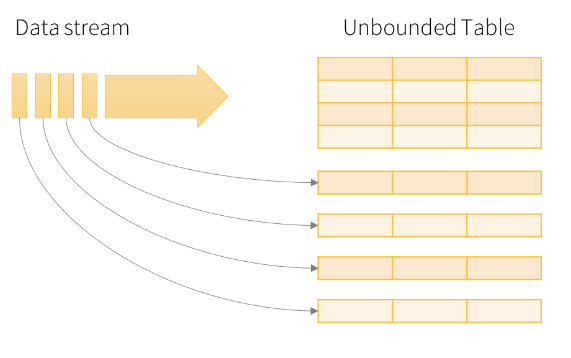
\includegraphics[width=\linewidth]{images/table.png}
  \end{column}
\end{columns}
\end{frame}


\begin{frame}\frametitle{Introducción - Modelo de programación declarativo}
	
\begin{itemize}
	\item \textbf{Se programa como en procesamiento en batch}
	\begin{itemize}
		\item API SQL/DataFrame con transformaciones encadenadas
		\item Misma lógica para datos finitos y para flujos continuos
	\end{itemize}

	\vspace{1em}

	\item \textbf{Modelo mental: tabla $\rightarrow$ query $\rightarrow$ salida}
	\begin{itemize}
		\item El \textit{stream} se interpreta como una tabla que crece
		\item La query produce resultados de forma incremental
	\end{itemize}

	\vspace{1em}

	\item \textbf{Enfoque declarativo}
	\begin{itemize}
		\item Defines \textit{qué} calcular, no los detalles de ejecución
		\item Spark planifica y optimiza el \textit{cómo}
	\end{itemize}
\end{itemize}
\end{frame}

\begin{frame}\frametitle{Introducción - DataFrames y Datasets}
	\begin{itemize}
		\item \textbf{Misma API que en batch}
		\begin{itemize}
			\item Operaciones habituales (\texttt{select}, \texttt{join}, \texttt{count}, ...)
			\item Permite reutilizar lógica batch en pipelines de streaming
		\end{itemize}

		\vspace{1em}

		\item \textbf{Particularidades en streaming}
		\begin{itemize}
			\item Resultados incrementales $\rightarrow$ la salida se actualiza con nuevos datos
			\item Gestión de estado $\rightarrow$ agregaciones/ventanas 
			\item Semánticas de salida $\rightarrow$ \textit{append}, \textit{update}, \textit{complete}
		\end{itemize}
	\end{itemize}
\end{frame}


\begin{frame}\frametitle{Introducción - Streaming query}
	\begin{itemize}
		\item \textbf{Consulta declarativa sobre un stream de eventos}
		\begin{itemize}
			\item Se expresa como una query de tipo batch (DataFrame/SQL)
			\item Se evalúa incrementalmente en cada trigger con los datos nuevos
			\item Spark SQL la planifica y optimiza (Catalyst + Tungsten)

		\end{itemize}

		\vspace{1em}

		\item \textbf{Los resultados se escriben en un destino de salida}

		\vspace{1em}

		\item \textbf{Ejemplos son resultados que se actualizan en cada trigger}
	\end{itemize}
\end{frame}

\begin{frame}\frametitle{Introducción - Streaming query}
	\centering
	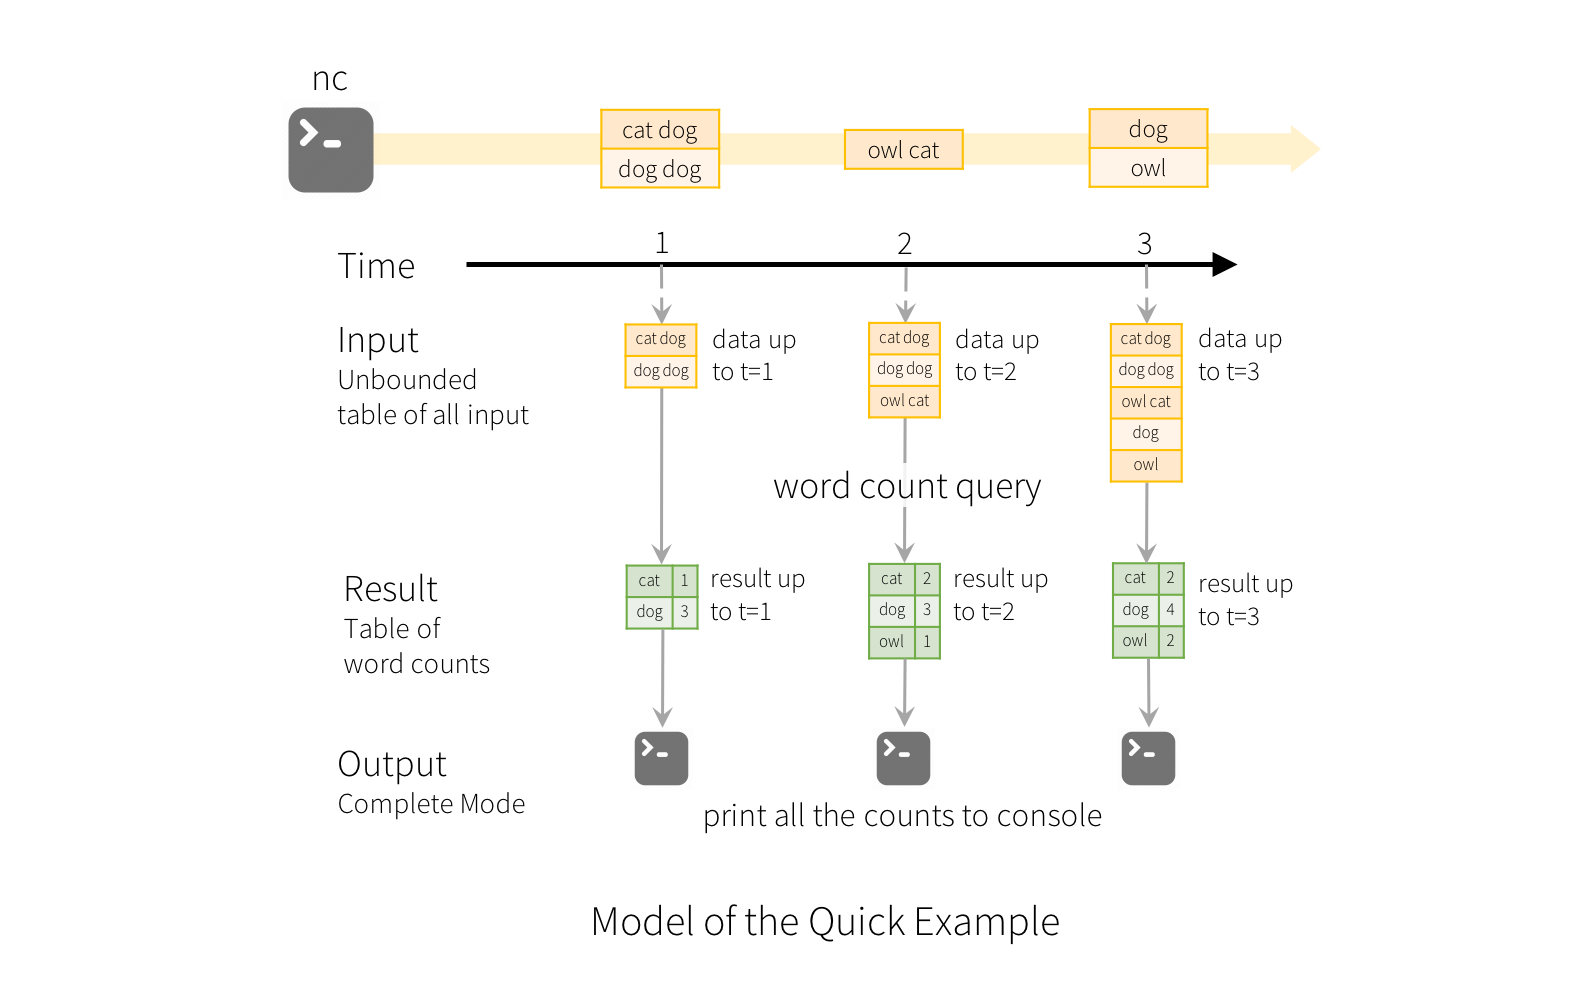
\includegraphics[width=0.8\linewidth]{images/word_count.png}
\end{frame}



\section{Componentes}

\begin{frame}\frametitle{Componentes - Arquitectura}
	\centering
	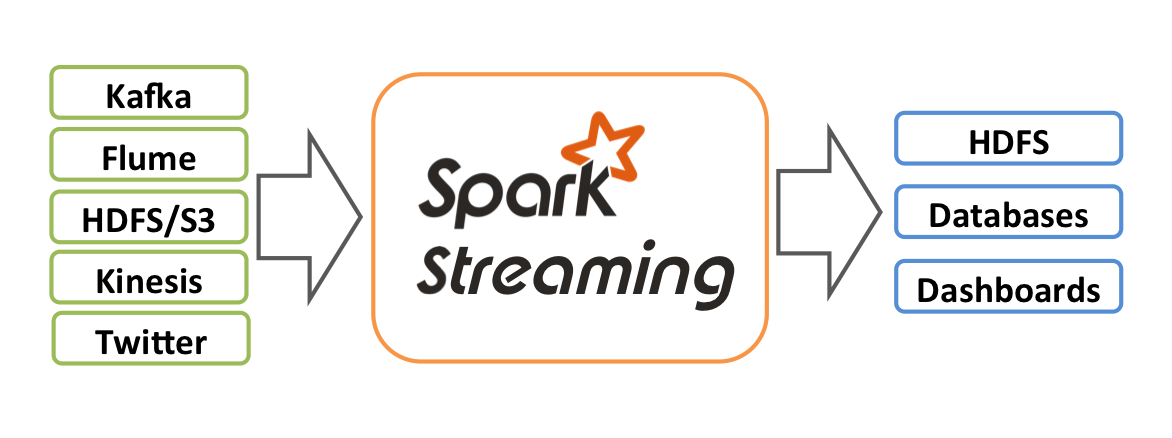
\includegraphics[width=0.9\linewidth]{images/streaming-arch.png}
	\centerline{\textbf{Entrada $\rightarrow$ Transformaciones (sin/con estado) $\rightarrow$ Salida}}
\end{frame}

\begin{frame}\frametitle{Componentes - Arquitectura}
	\centering
	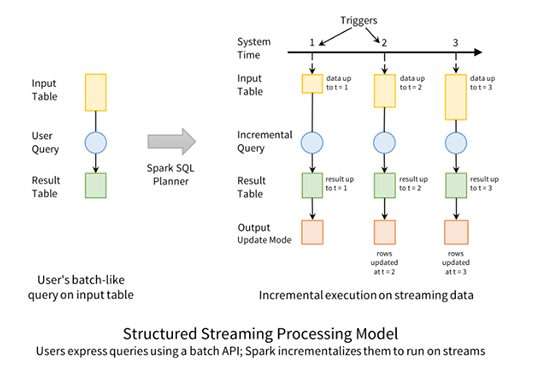
\includegraphics[width=0.65\linewidth]{images/structured-streaming.png}
\end{frame}

		\begin{frame}\frametitle{Introducción - SparkSession}
	\begin{itemize}
	\item \textbf{SparkSession es el punto de entrada}
	\begin{itemize}
		\item Las entradas (sources) se leen con \texttt{spark.readStream}
		\item Las salidas (sinks) se escriben con \texttt{df.writeStream}
	\end{itemize}

	\vspace{1em}

	\item \textbf{Del mismo stream se pueden ejecutar múltiples queries}
\begin{itemize}
		\item Query 1 $\rightarrow$ resultados por ventana (como posesión) para un dashboard
		\item Query 2 $\rightarrow$ detecta eventos críticos (posible lesión) y los publica en Kafka
	\end{itemize}
	\end{itemize}
\end{frame}


\begin{frame}\frametitle{Componentes - Fuentes de entrada (sources)}
\begin{columns}
  \begin{column}{0.55\textwidth}
    \begin{itemize}
      \item \textbf{Lectura de streams con \texttt{spark.readStream}}

      \vspace{1em}

      \item \textbf{Soporta múltiples fuentes habituales}
      \begin{itemize}
        \item Kafka como sistema de mensajería
        \item File para nuevos ficheros en un directorio
        \item Socket para pruebas rápidas (Netcat)
        \item Rate para testing y benchmarking
      \end{itemize}

      \vspace{1em}

      \item \textbf{El paralelismo suele venir de la fuente}
      \begin{itemize}
        \item Como particiones de tópicos de Kafka
        \item Más particiones $\Rightarrow$ más tareas en paralelo
      \end{itemize}
    \end{itemize}
  \end{column}
  \begin{column}{0.45\textwidth}
    \centering
    
\includegraphics[width=0.7\linewidth]{images/kafka.png}
  \end{column}
\end{columns}
\end{frame}


\begin{frame}\frametitle{Introducción - Query en streaming}
	\begin{itemize}
		\item \textbf{Control de ejecución de una query}
		\begin{itemize}
			\item \texttt{query = df.writeStream...\ .start()} inicia una query
			\item \texttt{query.awaitTermination()} bloquea hasta que termine
			\item \texttt{query.stop()} detiene la query (graceful stop)
		\end{itemize}
		\vspace{1em}
		\item \textbf{Operación de queries en producción}
		\begin{itemize}
			\item Poner un nombre descriptivo a la query
			\item Un mismo job (programa) puede ejecutar múltiples queries en paralelo
		\end{itemize}
	\end{itemize}
\end{frame}

\begin{frame}\frametitle{Componentes - Esquema y parsing}
	\begin{itemize}
		\item \textbf{En streaming el esquema es esencial}
		\begin{itemize}
			\item En un stream infinito no se recomienda inferir
			\item Es importante definir el esquema (JSON)
			\item Esto incluye tipar los campos de eventos
		\end{itemize}

		\vspace{1em}

		\item \textbf{Decisiones de parsing de eventos}
		\begin{itemize}
			\item Registros corruptos $\rightarrow$ enviar a cola aparte o fallar
			\item Evolución de esquema $\rightarrow$ versionado/validación
		\end{itemize}
	\end{itemize}
\end{frame}

\begin{frame}\frametitle{Componentes - Operaciones sin estado}
	\begin{itemize}
		\item \textbf{Operaciones sin recordar el pasado}
		\begin{itemize}
			\item Suelen escalar mejor $\rightarrow$ no requieren estado compartido entre micro-batches
			\item Algunas son \texttt{select}, \texttt{filter}, \texttt{withColumn}, \texttt{explode}, \texttt{map}, \dots
			\item Filtrar \texttt{event\_type == "SHOT"} o extraer minutos de un timestamp
		\end{itemize}
		\vspace{1em}
		\item \textbf{Si no hay agrupación/ventanas/join temporal/dedup normalmente es stateless}
	\end{itemize}
\end{frame}

\begin{frame}\frametitle{Componentes - Operaciones con estado}
	\begin{itemize}
		\item \textbf{Matienen el estado entre micro-batches}
		\begin{itemize}
			\item Recuerdan eventos anteriores
		\end{itemize}
		
		\vspace{1em}
	
		\item \textbf{Tipos de operaciones con estado}
		\begin{itemize}
			\item Agregaciones $\rightarrow$ \texttt{groupBy}, \texttt{count/sum/avg}
			\item Deduplicación  $\rightarrow$ \texttt{dropDuplicates}
			\item Joins  $\rightarrow$ stream-static y stream-stream
			\item Estado custom  $\rightarrow$ \texttt{mapGroupsWithState}
		\end{itemize}	
	\end{itemize}
\end{frame}

\begin{frame}\frametitle{Componentes - Operaciones con estado}
	\begin{itemize}
		\item \textbf{Propiedades a alto nivel}
		\begin{itemize}
			\item Estado actualizado incrementalmente entre micro-batches
			\item Recuperación y tolerancia a fallos mediante checkpointing
			\item Limpieza y estado acotado con watermarks o timeouts
		\end{itemize}

		\vspace{1em}

		\item \textbf{Ejemplo $\rightarrow$ resultados por ventanas de últimos 5 minutos}
	\end{itemize}
\end{frame}


\begin{frame}\frametitle{Componentes - Joins}
	\begin{itemize}
		\item \textbf{Stream-to-Static}
		\begin{itemize}
			\item Enriquecer un stream con datos (relativamente) estáticos
			\item Ejemplo $\rightarrow$ eventos del partido en streaming + datos de la plantilla
		\end{itemize}

		\vspace{1em}

		\item \textbf{Stream-to-Stream}
		\begin{itemize}
			\item Correlacionar eventos entre dos streams
			\item Requiere tiempo de evento + watermarks + rango temporal para acotar estado
			\item Ejemplo $\rightarrow$ eventos del partido + biometría en streaming
		\end{itemize}

		\vspace{1em}

	\item \textbf{Joins stream-stream sin cota temporal crecen el estado indefinidamente}
	\end{itemize}
\end{frame}


\begin{frame}\frametitle{Componentes - Tiempo de evento y proceso}
	\begin{itemize}
		\item \textbf{Eventos tardíos / fuera de orden}
		\begin{itemize}
			\item Cuando ocurrió $\neq$ Cuando llegó
			\item Ventanas/agregaciones usan tiempo de evento
			\item El trigger marca cada cuánto se procesa
		\end{itemize}

		\vspace{1em}

		\item \textbf{Watermark define la tardanza aceptada}
		\begin{itemize}
			\item Cierra ventanas y acota estado
			\item Define hasta cuándo se procesan eventos tardíos
		\end{itemize}
	\end{itemize}
\end{frame}

\begin{frame}\frametitle{Componentes - Ventanas}
\begin{columns}
  \begin{column}{0.5\textwidth}
    \begin{itemize}
      \item \textbf{Agrupaciones en intervalos de tiempo}

      \vspace{1em}

      \item \textbf{Ventanas fijas (tumbling)}
      \begin{itemize}
        \item Bloques fijos y no superpuestos
      \end{itemize}

      \vspace{1em}

      \item \textbf{Ventanas deslizantes (sliding)}
      \begin{itemize}
        \item Bloques que se superponen
      \end{itemize}

      \vspace{1em}

      \item \textbf{Ventanas de sesión (session)}
      \begin{itemize}
        \item Separados por gap de inactividad
      \end{itemize}

      \vspace{1em}

      \item \textbf{Es una columna más de agrupación}
    \end{itemize}
  \end{column}
  \begin{column}{0.52\textwidth}
    \centering
    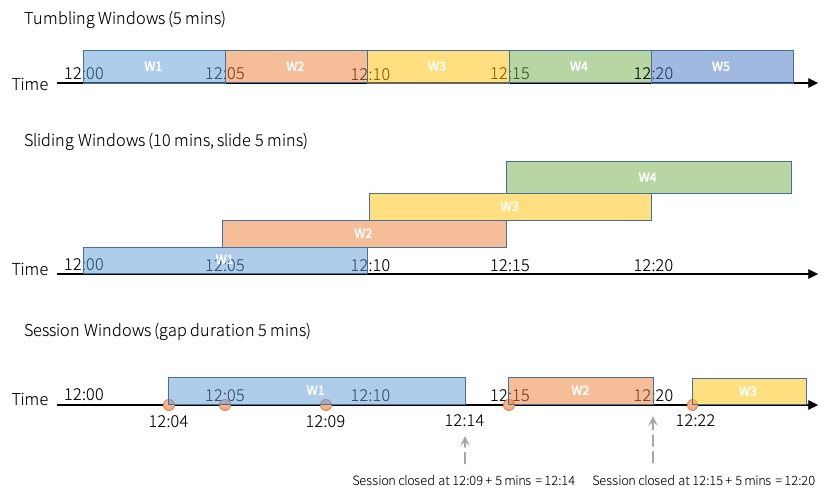
\includegraphics[width=\linewidth]{images/windows.jpg}
  \end{column}
\end{columns}
\end{frame}


\begin{frame}\frametitle{Componentes - Ventanas}
	\centering
	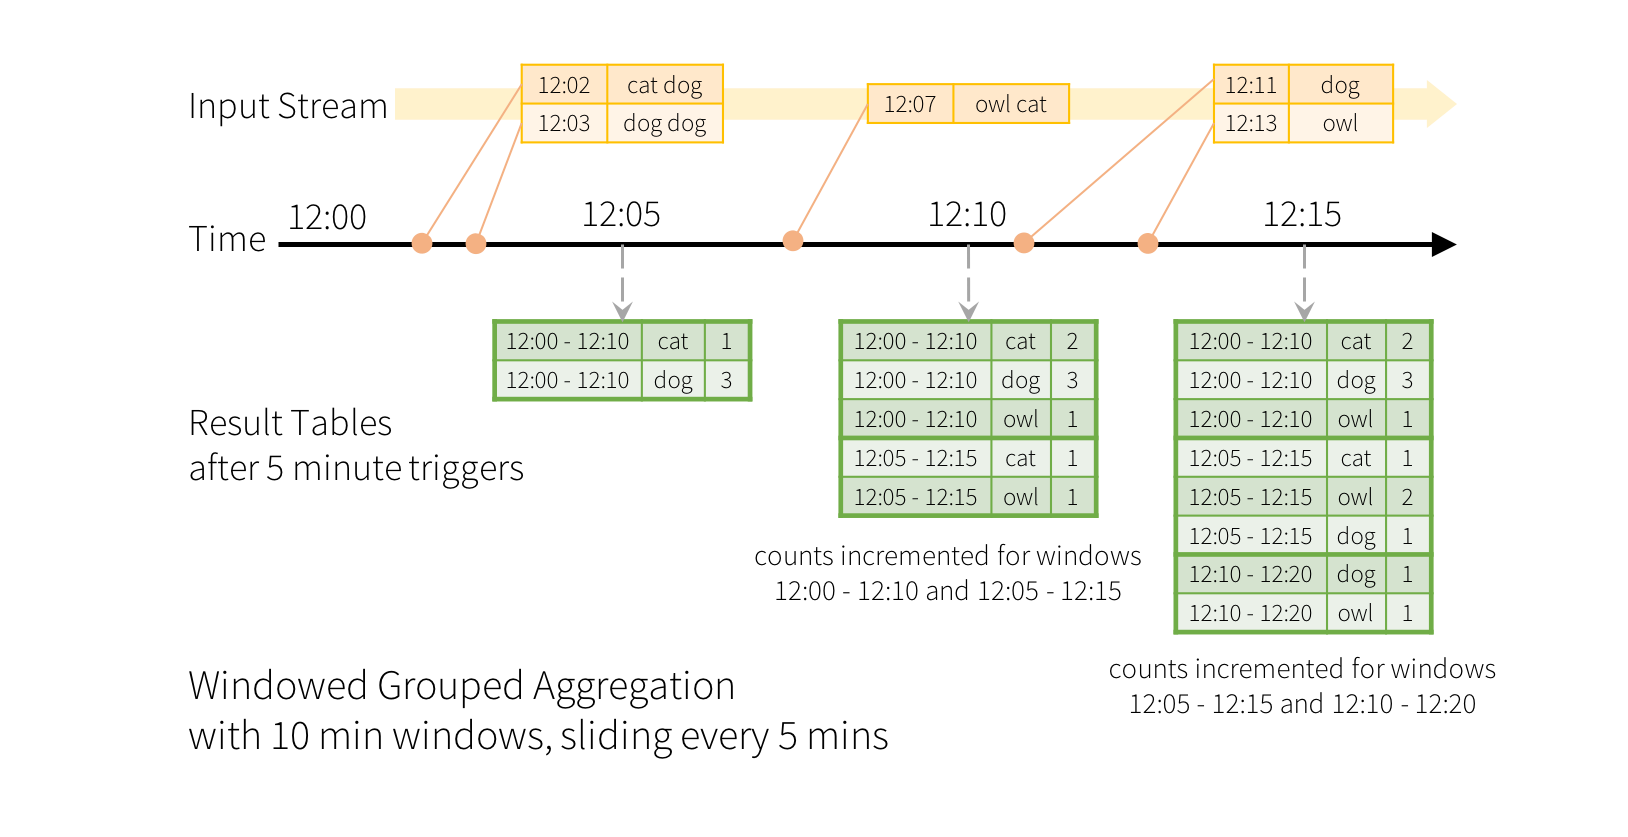
\includegraphics[width=0.8\linewidth]{images/window.png}
\end{frame}

\begin{frame}\frametitle{Componentes - Trigger}
	\begin{itemize}
		\item \textbf{Define cada cuánto se ejecuta la query para procesar nuevos datos}
		\begin{itemize}
			\item Default $\rightarrow$ tan rápido como sea posible (micro-batch)
			\item ProcessingTime $\rightarrow$ intervalo fijo (por ejemplo cada 10s)
			\item AvailableNow $\rightarrow$ procesa lo disponible y se detiene
			\item Continuous $\rightarrow$ sólo en modo continuous (con restricciones)
		\end{itemize}
	\end{itemize}
\end{frame}

\begin{frame}\frametitle{Componentes - Watermarks}
	\begin{itemize}
		\item \textbf{Define cuánto esperar un evento tardío}
		\begin{itemize}
			\item Los eventos no siempre llegan en orden ni a tiempo
			\item El GPS de un jugador puede llegar 2 minutos tarde al servidor
			\item El watermark define cuánto retraso toleramos antes de cerrar una ventana
		\end{itemize}

		\vspace{1em}

		\item \textbf{Su uso es fundamental para controlar el estado}
		\begin{itemize}
			\item Un watermark de 2 minutos (tiempo de evento) acepta tardíos hasta 2 min
			\item Más allá los tardíos no actualizan ventanas/estado
		\end{itemize}

		\vspace{1em}

		\item \textbf{Supone un trade-off}
		\begin{itemize}
			\item Watermark amplio $\rightarrow$ más precisión pero más memoria usada
			\item Watermark corto $\rightarrow$ resultados más rápidos pero posibles eventos perdidos
		\end{itemize}
	\end{itemize}
\end{frame}

\begin{frame}\frametitle{Componentes - Late data}
	\begin{itemize}
		\item \textbf{Es habitual que lleguen eventos tardíos}
		\begin{itemize}
			\item Dentro del watermark $\rightarrow$ se incluye en el cálculo y puede corregir un resultado emitido
			\item Fuera del watermark $\rightarrow$ se descarta para mantener los resultados estables
		\end{itemize}

		\vspace{1em}

		\item \textbf{Ejemplo $\rightarrow$ tiros a puerta en los últimos 5 minutos}
		\begin{itemize}
			\item Un sensor registra un tiro a las 18:32 pero el dato llega a las 18:34
			\item Con watermark de 3 minutos $\rightarrow$ se acepta y corrige del intervalo 18:30--18:35
			\item Con watermark de 1 minuto $\rightarrow$ llega demasiado tarde y se descarta
		\end{itemize}
	\end{itemize}
\end{frame}

\begin{frame}\frametitle{Componentes - Late data}
	\centering
	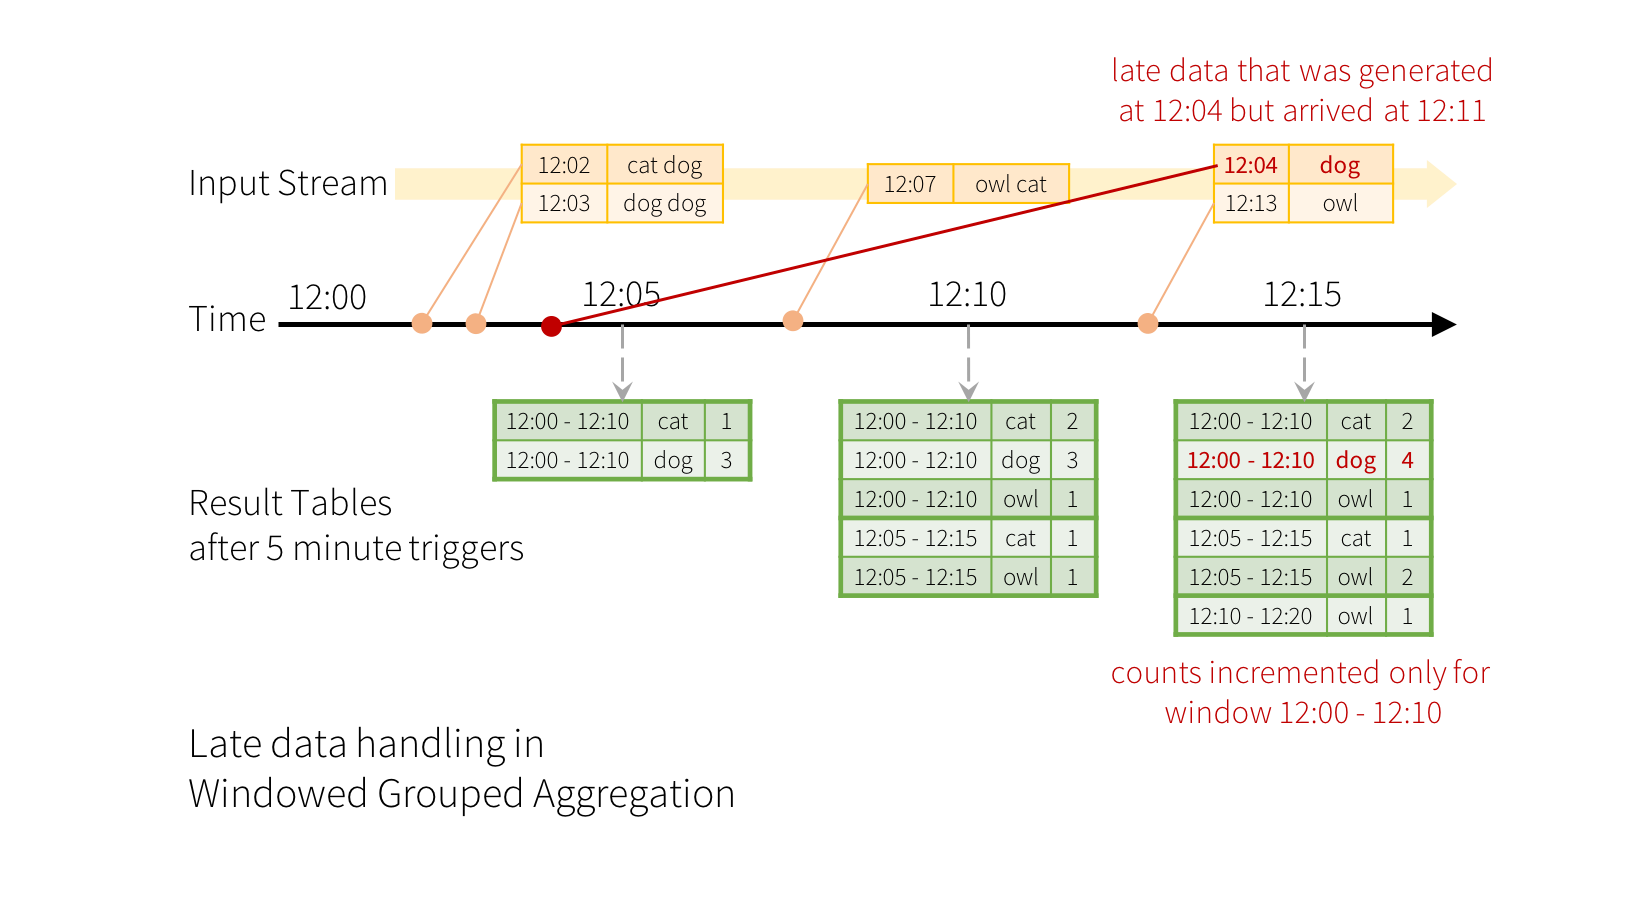
\includegraphics[width=0.8\linewidth]{images/late_data.png}
\end{frame}




\begin{frame}\frametitle{Componentes - Semánticas de escritura}
	\begin{itemize}
		\item \textbf{Append escribe solo filas nuevas y finales}
		\begin{itemize}
			\item No reescribe filas
			\item En ventanas emite cuando la ventana se “cierra”
			\item Útil para eventos crudos o resultados finales
		\end{itemize}

		\vspace{1em}

		\item \textbf{Update escribe filas que cambian}
		\begin{itemize}
			\item Reescribe solo las filas actualizadas desde el último trigger
			\item Útil para resultados en vivo (contadores en evolución)
		\end{itemize}

		\vspace{1em}
			
		\item \textbf{Complete reescribe la \textbf{tabla completa} en cada trigger}
		\begin{itemize}
			\item Solo viable si la tabla de resultados es pequeña
		\end{itemize}
	\end{itemize}
\end{frame}


\begin{frame}\frametitle{Componentes - Semánticas de escritura}
	\centering
	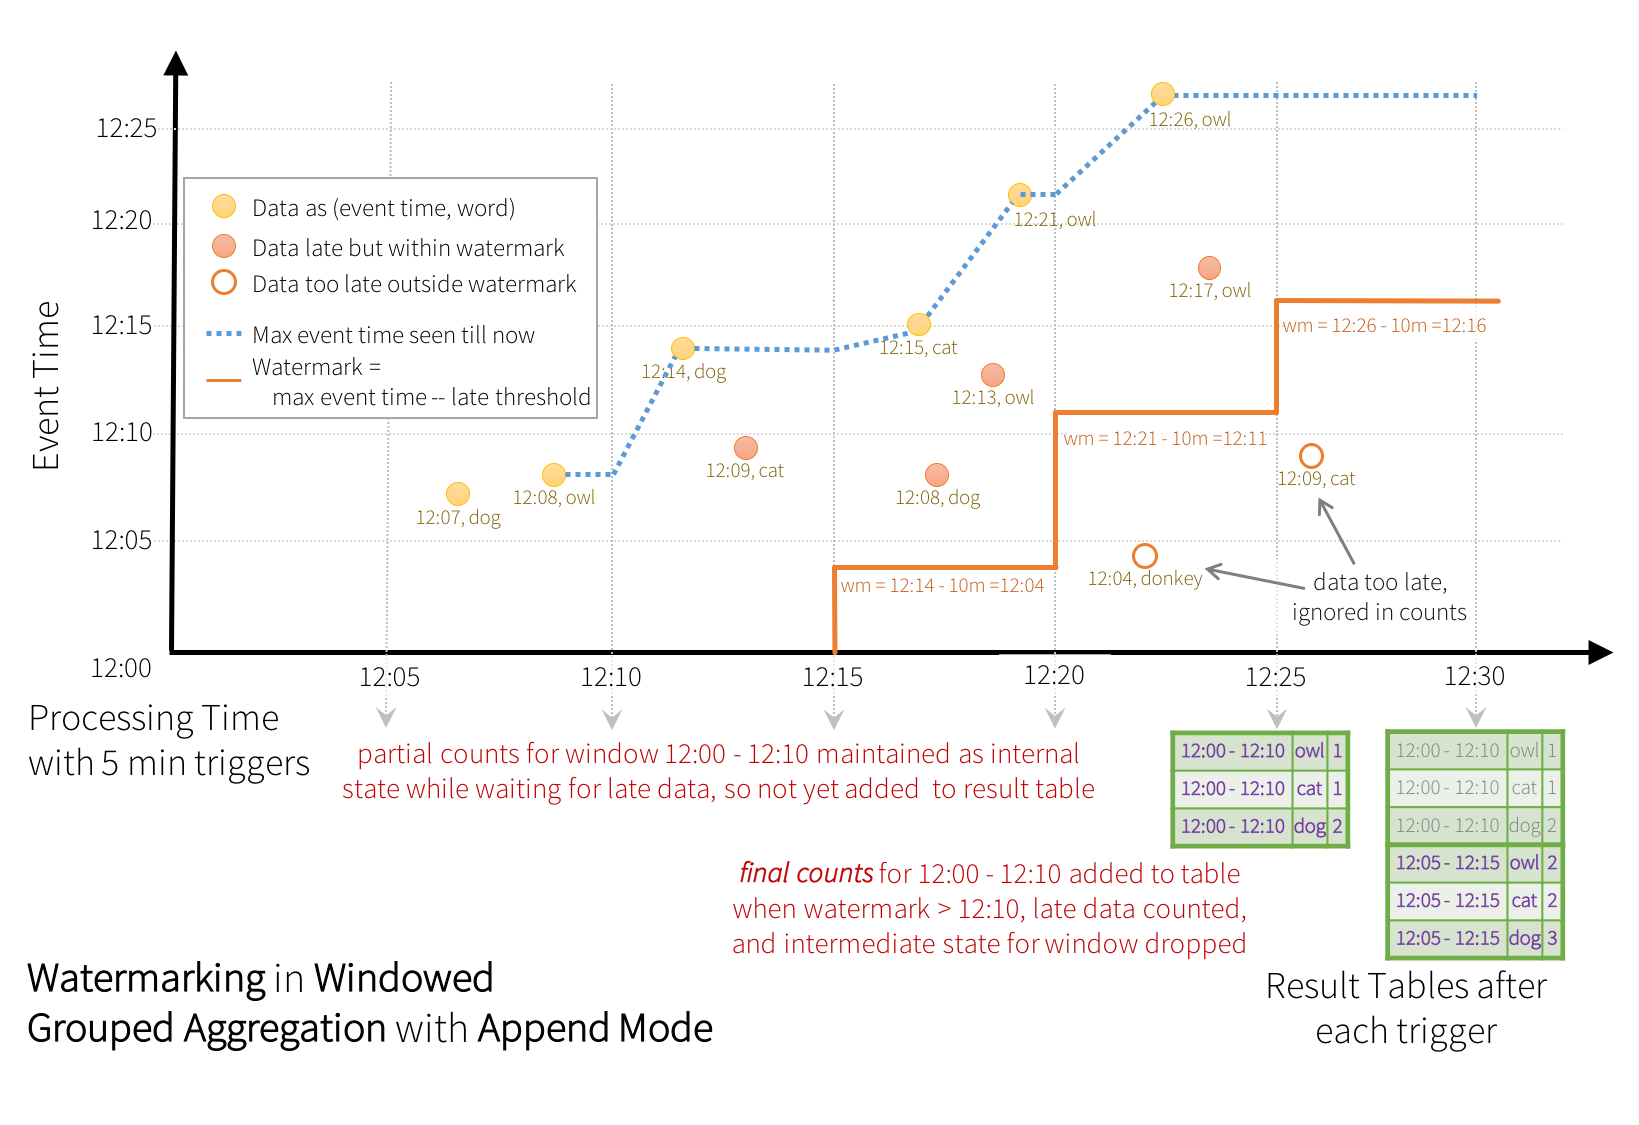
\includegraphics[width=0.65\linewidth]{images/watermark_append.png}
\end{frame}


\begin{frame}\frametitle{Componentes - Semánticas de escritura}
	\centering
	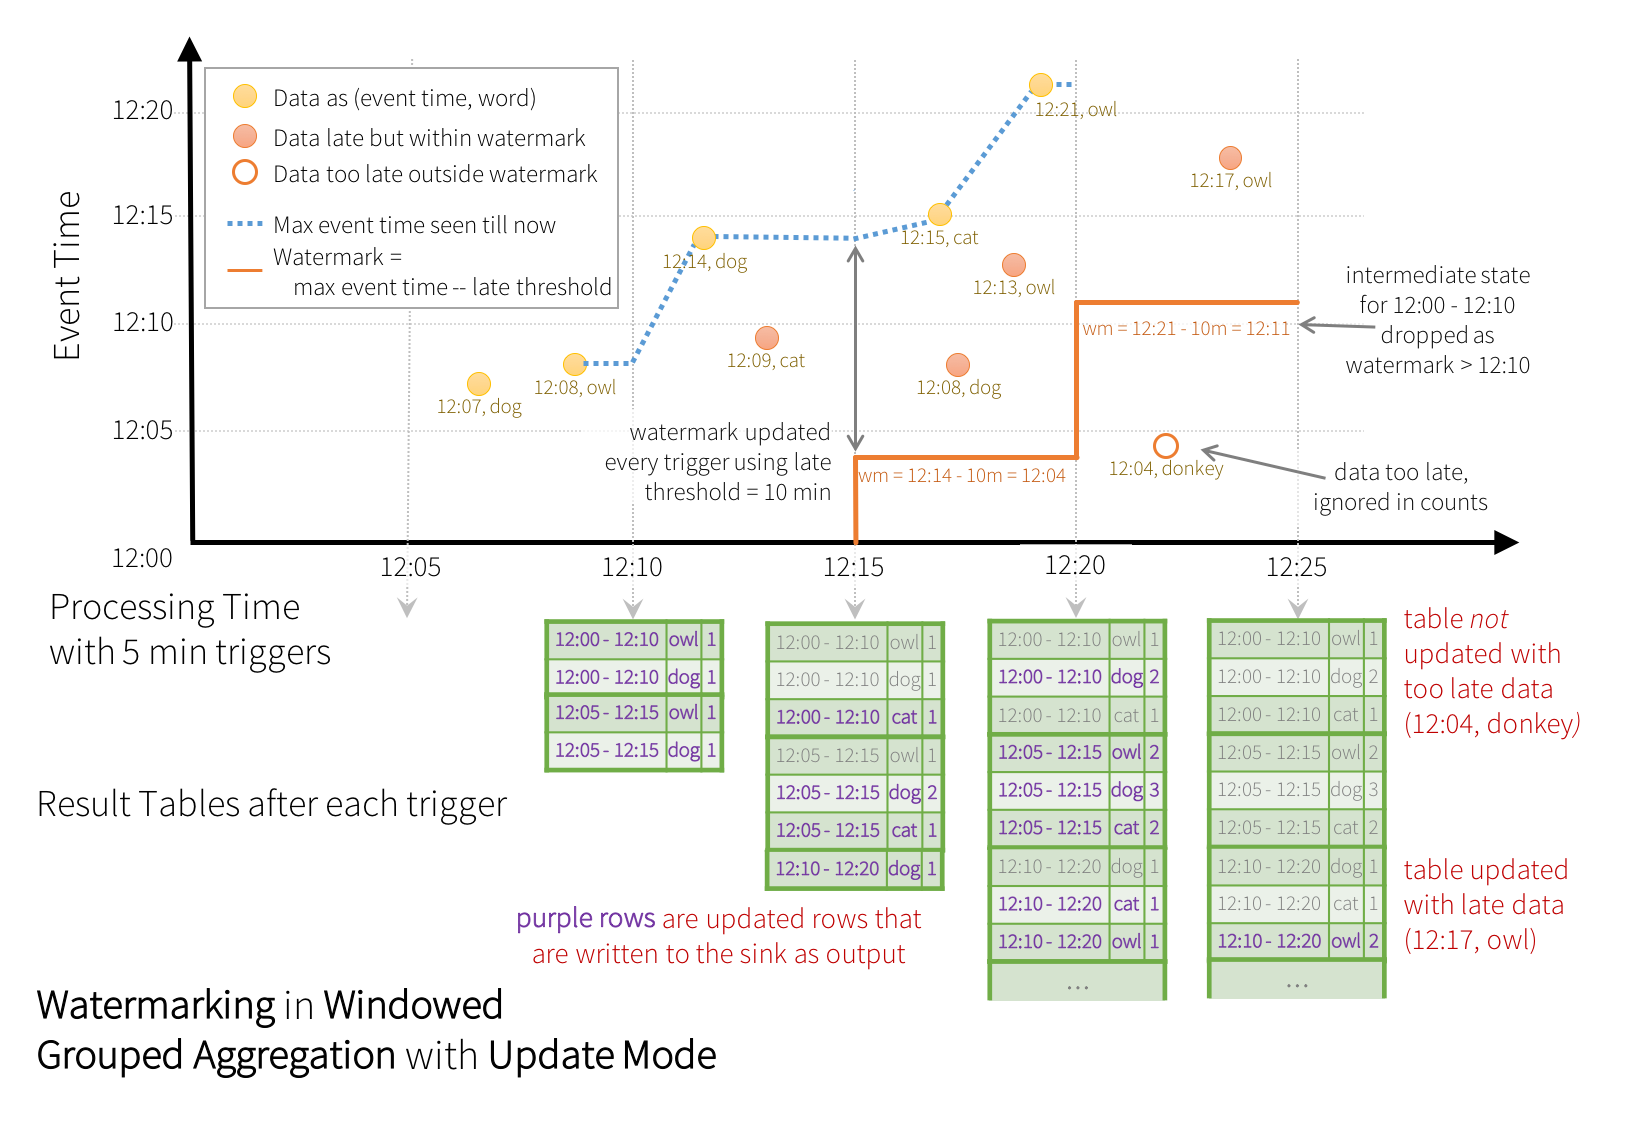
\includegraphics[width=0.65\linewidth]{images/watermark_update.png}
\end{frame}


\begin{frame}\frametitle{Componentes - Destinos de salida (sinks)}
\begin{columns}
  \begin{column}{0.55\textwidth}
    \begin{itemize}
      \item \textbf{Escritura de resultados con \texttt{writeStream}}

      \vspace{1em}

      \item \textbf{Soporta múltiples destinos habituales}
      \begin{itemize}
        \item Sistemas de mensajería (Kafka)
        \item Bases de datos SQL y NoSQL (InfluxDB)
        \item Archivos como HDFS/S3 (Parquet/JSON)
        \item Consola/memoria para depuración y desarrollo
        \item \texttt{foreach}/\texttt{foreachBatch} para lógica personalizada
      \end{itemize}
    \end{itemize}
  \end{column}
  \begin{column}{0.45\textwidth}
    \centering
    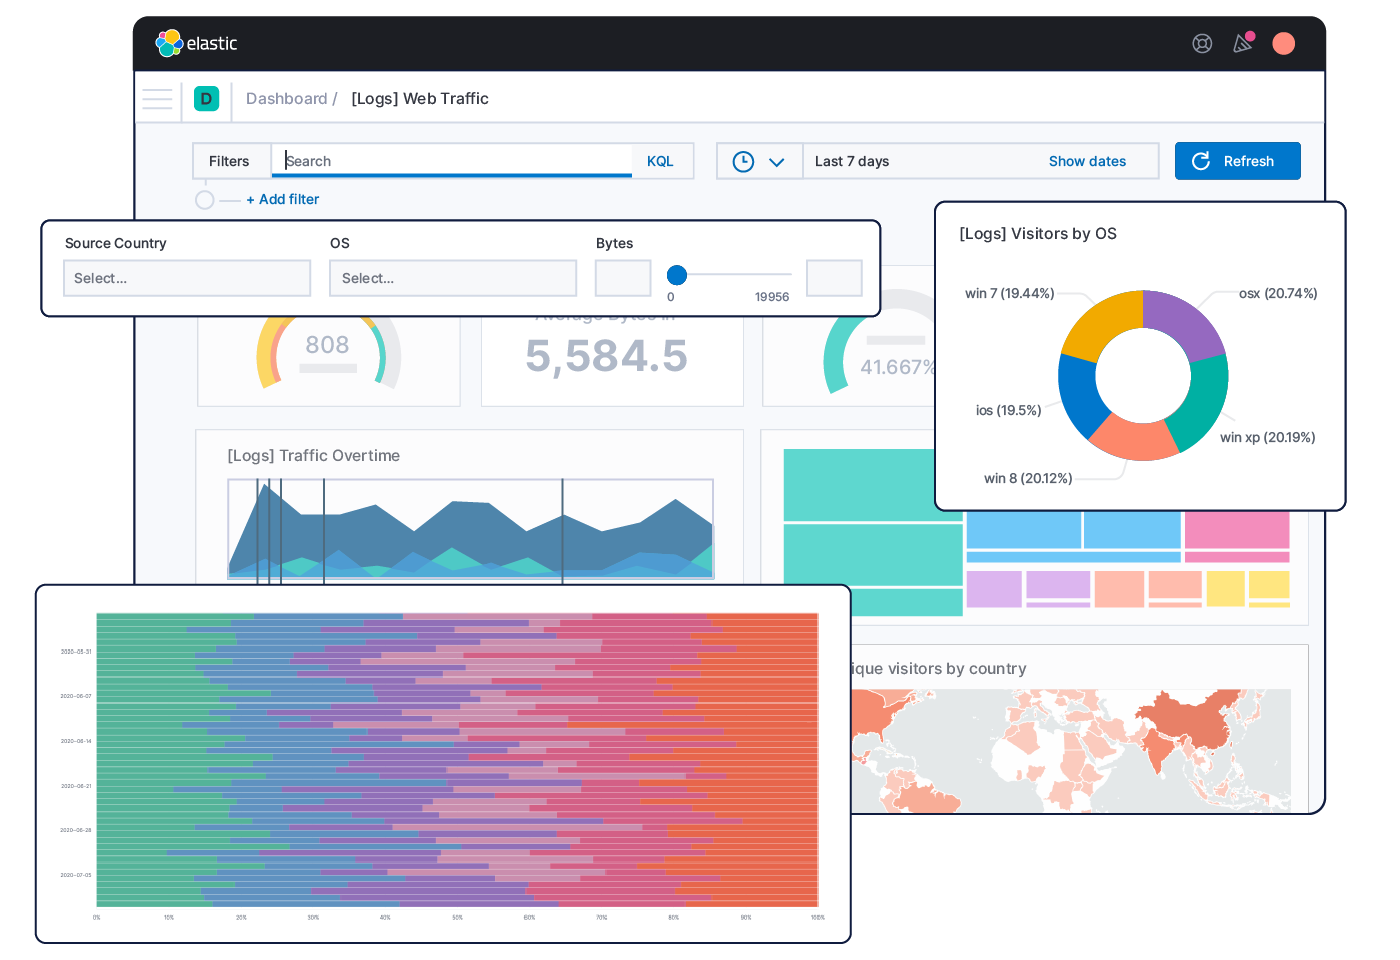
\includegraphics[width=\linewidth]{images/kibana.png}
  \end{column}
\end{columns}
\end{frame}



\section{Infraestructura}

\begin{frame}\frametitle{Infraestructura - Deduplication}
	\begin{itemize}
		\item \textbf{Eliminar duplicados en streaming}
		\begin{itemize}
			\item La fuente puede reemitir eventos (retries, reconexiones, \textit{at-least-once})
			\item Se deduplica por una clave estable (como \texttt{event\_id})
			\item Se usa watermark $\rightarrow$ limita cuánto tiempo recordamos
		\end{itemize}
	\end{itemize}
\end{frame}

\begin{frame}\frametitle{Infraestructura - Estado es un coste}
\begin{itemize}
	\item \textbf{Las operaciones con estado consumen recursos}
	\begin{itemize}
		\item Spark necesita recordar eventos pasados para calcular agregaciones y ventanas
		\item Más claves de agrupación o ventanas más amplias $\Rightarrow$ más memoria necesaria
	\end{itemize}

	\vspace{1em}

	\item \textbf{El watermark limita cuánto estado se acumula}
	\begin{itemize}
		\item Permite a Spark olvidar ventanas ya cerradas
		\item Sin watermark el estado crece indefinidamente
	\end{itemize}

	\vspace{1em}

	\item \textbf{Regla práctica: agrupa por pocas claves y usa ventanas razonables}
\end{itemize}
\end{frame}

\begin{frame}\frametitle{Infraestructura - Frescura de los datos}
	\begin{itemize}
		\item \textbf{El trigger controla cada cuánto se actualizan los resultados}
		\begin{itemize}
			\item Trigger corto $\rightarrow$ datos más frescos pero más carga en el sistema
			\item Trigger largo $\rightarrow$ datos menos frescos pero menos carga
		\end{itemize}

		\vspace{1em}

		\item \textbf{Regla práctica: elige el trigger según la necesidad del análisis}
		\begin{itemize}
			\item Dashboard en tiempo real $\rightarrow$ trigger de segundos
			\item Reporte por minuto $\rightarrow$ trigger de 60s es suficiente
		\end{itemize}
	\end{itemize}
\end{frame}

\begin{frame}\frametitle{Infraestructura - Checkpointing}
	\begin{itemize}
		\item \textbf{Spark recuerda hasta dónde llegó}
		\begin{itemize}
			\item Guarda un punto de control tras cada micro-batch
			\item Si el proceso cae, retoma desde ahí sin reprocesar datos ya calculados
			\item Evita duplicados y pérdida de resultados intermedios
		\end{itemize}

		\vspace{1em}

		\item \textbf{Checkpointing para recuperación tras fallos}
		\begin{itemize}
			\item Persiste progreso y estado
			\item Spark persiste logs de progreso/commits asociados a cada trigger
			\item Tras un reinicio reanuda desde el último progreso consistente
		\end{itemize}
	\end{itemize}
\end{frame}



\begin{frame}\frametitle{Infraestructura - Garantía Exactly-Once}
	\begin{itemize}
		\item \textbf{Spark garantiza que cada evento se procesa exactamente una vez}
		\begin{itemize}
			\item Los resultados no se duplican ni se pierden aunque el sistema falle y se reinicie
		\end{itemize}

		\vspace{1em}

		\item \textbf{Para que funcione se necesitan tres condiciones}
		\begin{itemize}
			\item La fuente permite releer datos (como Kafka)
			\item Spark guarda el progreso (checkpointing)
			\item El destino tolera escrituras duplicadas sin problemas
		\end{itemize}
	\end{itemize}
\end{frame}


\section{Ejemplos}

\begin{frame}[fragile]\frametitle{Ejemplos - Spark en local}
\begin{itemize}
	\item \textbf{Se recomienda despliegue local / Docker para pruebas}

	\vspace{1em}

	\item \textbf{Requisitos de instalación en despliegue local de Spark}
	\begin{itemize}
		\item Java instalado (\texttt{java -{}-version}) y configurar \texttt{JAVA\_HOME}
		\item Instalar PySpark y crear una sesión local con todos los núcleos \texttt{[*]}
	\end{itemize}
\end{itemize}

\vspace{1em}

\begin{shellbox}
\begin{shcode}
java --version                     # verificar Java
apt install -y openjdk-21-jdk      # instalar Java (Colab / Linux)
pip install pyspark                # instalar PySpark
\end{shcode}
\end{shellbox}
\end{frame}



\begin{frame}[fragile]\frametitle{Ejemplos - Spark en local}
\begin{itemize}
  \item \textbf{Si \texttt{JAVA\_HOME} no está definida hay que indicarla manualmente}
\end{itemize}

\vspace{0.5em}

\begin{code}
\begin{python3code}
import os
import pyspark

# En Debian/Ubuntu con version 21 de Java:
# os.environ["JAVA_HOME"] = "/usr/lib/jvm/java-21-openjdk-amd64"
# En Windows con version 21 de Java:
# os.environ["JAVA_HOME"] = "C:\\Program Files\\Java\\jdk-21"

print(os.environ["JAVA_HOME"])   # comprobar si esta definida
print(pyspark.__version__)
\end{python3code}
\end{code}
\end{frame}


\begin{frame}[fragile]\frametitle{Ejemplos - Spark con Docker}
\begin{itemize}
	\item \textbf{Jupyter + PySpark ya instalados y configurados}
\end{itemize}

\vspace{2em}

\begin{shellbox}
\begin{shcode}
docker run \
 --network=host \
 -e JUPYTER_TOKEN="MY_SECRET" \
 -v ${PWD}:/home/jovyan/work \
 jupyter/pyspark-notebook
\end{shcode}
\end{shellbox}
\end{frame}


\begin{frame}[fragile]\frametitle{Ejemplos - Spark con Docker Compose}
\begin{shcode}
    services:
      jupyter:
        image: jupyter/pyspark-notebook
        network_mode: host
        environment:
          - JUPYTER_TOKEN=MY_SECRET
        restart: on-failure
        volumes:
          - ./:/home/jovyan/work
\end{shcode}
\end{frame}


\begin{frame}[fragile]\frametitle{Ejemplos - Contar tipos de eventos de un partido}

\begin{enumerate}
  \item \textbf{Leer líneas Spark desde un socket en el puerto 9999}
  \begin{itemize}
	\item Cada línea representa un evento de un partido de fútbol
	\item Pueden ser \texttt{goal}, \texttt{shot}, \texttt{foul} y \texttt{pass}
  \end{itemize}

  \vspace{1em}

  \item \textbf{Filtrar solo eventos válidos y normalizar cada línea}

  \vspace{1em}

  \item \textbf{Agregar el conteo acumulado por tipo de evento}
  
  \vspace{1em}

  \item \textbf{Escribir los resultados en consola}
\end{enumerate}
\end{frame}

\begin{frame}[fragile]\frametitle{Ejemplos - Contar tipos de eventos de un partido}

\begin{itemize}
	\item \textbf{Paso 0 - Simular un flujo de tipos de eventos de un partido de fútbol}
	\begin{itemize}
		\item Socket con Netcat para enviar eventos de prueba
		\item En Windows instalar Nmap (https://nmap.org/download)
	\end{itemize}
\end{itemize}

\vspace{1em}

\begin{shellbox}
\begin{shcode}
# En local
nc -lv 9999

# En docker
docker run --rm -it --init -p 9999:9999 madrueno/nc -lv 9999
\end{shcode}
\end{shellbox}
\end{frame}

\begin{frame}[fragile]\frametitle{Ejemplos - Contar tipos de eventos de un partido}

\begin{itemize}
	\item \textbf{Paso 1 - Iniciar una sesión de Spark Structured Streaming}
\end{itemize}

\vspace{1em}

\begin{code}
\begin{python3code}
from pyspark.sql import SparkSession
from pyspark.sql.functions import col, lower, trim

spark = (
    SparkSession.builder					# Construye la sesión de Spark
    .appName("FootballStreamingEventCount") # Nombre descriptivo
    .getOrCreate()						  # Crea o reutiliza la sesión existente
)
\end{python3code}
\end{code}
\end{frame}

\begin{frame}[fragile]\frametitle{Ejemplos - Contar tipos de eventos de un partido}

\begin{itemize}
	\item \textbf{Paso 2 - Leer líneas de eventos desde el socket abierto}
\end{itemize}

\vspace{1em}

\begin{code}
\begin{python3code}
lines = (
    spark.readStream		     # Lee un stream de una fuente
    .format("socket")			# Fuente de tipo socket
    .option("host", "localhost") # Host del socket
    .option("port", 9999)		# Puerto del socket
    .load()					  # Carga como DataFrame
)
\end{python3code}
\end{code}
\end{frame}

\begin{frame}[fragile]\frametitle{Ejemplos - Contar tipos de eventos de un partido}

\begin{itemize}
	\item \textbf{Paso 3 - Normalizar texto y filtrar eventos válidos}
	\begin{itemize}
		\item Convertir a minúsculas y eliminar espacios
		\item Filtrar solo los tipos de eventos de interés
	\end{itemize}
\end{itemize}

\vspace{1em}

\begin{code}
\begin{python3code}
valid = ["goal", "shot", "foul", "pass"] 			 # Tipos de eventos válidos

events = (
    lines											 # DataFrame (string por defecto)
    .select(trim(lower(col("value"))).alias("event")) # Normaliza texto
    .where(col("event").isin(valid))				  # Filtra solo eventos válidos
)
\end{python3code}
\end{code}
\end{frame}



\begin{frame}[fragile]\frametitle{Ejemplos - Contar tipos de eventos de un partido}

\begin{itemize}
	\item \textbf{Paso 4 - Agregar el conteo acumulado por tipo de evento}
	\begin{itemize}
		\item Agrupa por tipo y cuenta el número de eventos por tipo
		\item La query no se ejecuta hasta que se escriba la salida
	\end{itemize}
\end{itemize}

\vspace{1em}

\begin{code}
\begin{python3code}
counts = (
    events			 # DataFrame con eventos
    .groupBy("event")  # Agrupa por tipo de evento
    .count()		   # Cuenta el número de eventos por tipo
)
\end{python3code}
\end{code}
\end{frame}


\begin{frame}[fragile]\frametitle{Ejemplos - Contar tipos de eventos de un partido}

\begin{itemize}
	\item \textbf{Paso 5 - Escribir resultados continuamente en consola}
\end{itemize}

\vspace{1em}

\begin{code}
\begin{python3code}
query = (
    counts.writeStream        # Define el destino de salida
    .outputMode("complete")   # Muestra la tabla completa de conteos
    .format("console")        # Escribe en consola
    .start()                  # Inicia la query de streaming
)

query.awaitTermination()      # Espera hasta que se detenga la query
\end{python3code}
\end{code}
\end{frame}


\begin{frame}[fragile]\frametitle{Ejemplos - Contar acciones de gol por ventana}

\begin{itemize}
	\item \textbf{Entradas de prueba enviadas por netcat}
	\begin{itemize}
		\item Eventos con timestamp, equipo, tipo de evento y xG
		\item Se define un esquema explícito para parsear el JSON
		\item El campo \texttt{ts} permite aplicar ventanas temporales y watermark
	\end{itemize}
\end{itemize}

\vspace{1em}

\begin{shellbox}
\begin{shcode}
{"ts": "2025-06-01 10:00:10", "team": "RMA", "event": "goal", "xg": 0.9}
{"ts": "2025-06-01 10:00:40", "team": "FCB", "event": "shot", "xg": 0.2}
{"ts": "2025-06-01 10:02:55", "team": "RMA", "event": "shot", "xg": 0.3}
{"ts": "2025-06-01 09:45:40", "team": "FCB", "event": "shot", "xg": 0.2}
\end{shcode}
\end{shellbox}

\end{frame}



\begin{frame}[fragile]\frametitle{Ejemplos - Contar acciones de gol por ventana}

\begin{code}
\begin{python3code}
from pyspark.sql import SparkSession
from pyspark.sql import functions as F
from pyspark.sql.types import (
    StructType, StructField,
    StringType, DoubleType, TimestampType
)

spark = (
    SparkSession.builder
    .appName("FootballStreamingGoalEvents")
    .getOrCreate()                           
)
\end{python3code}
\end{code}
\end{frame}


\begin{frame}[fragile]\frametitle{Ejemplos - Contar acciones de gol por ventana}

\begin{itemize}
	\item \textbf{Definir el esquema explícito del evento JSON}
	\begin{itemize}
		\item Cada línea del socket es un objeto JSON con 4 campos
	\end{itemize}
\end{itemize}

\vspace{1em}

\begin{code}
\begin{python3code}
schema = StructType([
    StructField("ts",    TimestampType()), # Timestamp del evento
    StructField("team",  StringType()),    # Equipo que realizó la acción
    StructField("event", StringType()),    # Tipo de evento (goal, shot, etc.)
    StructField("xg",    DoubleType()),    # Goles esperados del evento
])
\end{python3code}
\end{code}
\end{frame}

\begin{frame}[fragile]\frametitle{Ejemplos - Contar acciones de gol por ventana}

\begin{itemize}
	\item \textbf{Leer y parsear eventos JSON desde el socket}
	\begin{itemize}
		\item Cada línea recibida se parsea con el esquema definido
	\end{itemize}
\end{itemize}

\vspace{1em}

\begin{code}
\begin{python3code}
events = (
    spark.readStream
    .format("socket")
    .option("host", "localhost")
    .option("port", 9999)
    .load()                                          # Columna "value" con el JSON crudo
    .select(F.from_json("value", schema).alias("e")) # Parsea JSON con el schema
    .select("e.*")                                   # Desempaqueta los campos
)
\end{python3code}
\end{code}
\end{frame}

\begin{frame}[fragile]\frametitle{Ejemplos - Contar acciones de gol por ventana}

\begin{itemize}
	\item \textbf{Aplicar watermark y agregar en ventanas}
	\begin{itemize}
		\item Tomamos ventanas de 1 minuto a modo de ejemplo
		\item El watermark descarta eventos que llegan con más de 2 minutos de retraso
		\item La ventana fija agrupa en bloques de 1 minuto según el timestamp del evento
	\end{itemize}
\end{itemize}

\vspace{1em}

\begin{code}
\begin{python3code}
counts = (
    events
	.filter(F.col("event").isin("goal", "shot")) # Filtra solo acciones de gol
    .withWatermark("ts", "5 minutes")            # Descarta eventos muy tardíos
    .groupBy(F.window("ts", "1 minute"), "team") # Ventana de 1 min por equipo
    .agg(F.count("*").alias("total"))            # Cuenta acciones por ventana
)
\end{python3code}
\end{code}
\end{frame}

\begin{frame}[fragile]\frametitle{Ejemplos - Contar acciones de gol por ventana}

\begin{itemize}
	\item \textbf{Escribir resultados en consola con trigger periódico}
	\begin{itemize}
		\item El trigger actualiza los resultados cada 10 segundos
	\end{itemize}
\end{itemize}

\vspace{1em}

\begin{code}
\begin{python3code}
query = (
    counts.writeStream)
    .outputMode("update")                   # Emite resultados actualizados
    .format("console")                      
    .trigger(processingTime="10 seconds")   # Ejecuta un micro-batch cada 10 s
    .start()                              
)

query.awaitTermination()
\end{python3code}
\end{code}
\end{frame}

\begin{frame}[fragile]\frametitle{Ejemplos - Contar acciones de gol por ventana}

\begin{itemize}
	\item \textbf{Enviar eventos con timestamps desordenados}
\end{itemize}

\vspace{0.5em}

\begin{shellbox}
\begin{shcode}
# Batch 1 de eventos
{"ts": "2025-06-01 10:00:10", "team": "RMA", "event": "goal", "xg": 0.9}
{"ts": "2025-06-01 10:00:40", "team": "FCB", "event": "shot", "xg": 0.2}
{"ts": "2025-06-01 10:02:55", "team": "RMA", "event": "shot", "xg": 0.3}
\end{shcode}
\end{shellbox}

\begin{shellbox}
\begin{shcode}
# Evento tardío (llega después pero ocurrió antes)
{"ts": "2025-06-01 09:45:40", "team": "FCB", "event": "shot", "xg": 0.2}
\end{shcode}
\end{shellbox}
\end{frame}


\begin{frame}\frametitle{Conclusiones}
	\begin{itemize}
		\item \textbf{Spark Structured Streaming para análisis en tiempo real}
		\begin{itemize}
			\item Unifica batch y streaming con un modelo declarativo
			\item Actualiza resultados incrementalmente y gestiona estado, tardíos
		\end{itemize}

		\vspace{1em}

		\item \textbf{Checklist práctico de desarrollo}
		\begin{itemize}
			\item Establecer fuente y definir el esquema de eventos
			\item Identificar tiempo de evento y configurar watermarks/ventanas
			\item Escoger destino y modo de escritura según necesidad
			\item Definir trigger para controlar frescura de resultados
			\item Ejecutar \texttt{start()} y \texttt{awaitTermination()}
		\end{itemize}
	\end{itemize}
\end{frame}

\end{document}
